\documentclass[10pt]{beamer}

\usepackage[utf8]{inputenc}
\usepackage{tcolorbox}
\usepackage{tikz}
\usepackage{tikz-3dplot}
\usetikzlibrary{intersections,calc}
\usepackage{amsmath}
\usepackage{graphicx}
\usepackage{cases}
\def \heart {\textcolor{blue}{$\heartsuit$} }
\def \C {$\mathcal{C}$}
\def \orthog {\underline{\perp}}
\def\arcos{\operatorname{arcos}}

\tcbset{%
	basic/.style={colframe=black,
		      colback=white,
		      top= 0mm,
		      bottom = 2mm,
		      boxsep=0mm
		      }
}
\tikzset{
    invisible/.style={opacity=0},
    visible on/.style={alt={#1{}{invisible}}},
    alt/.code args={<#1>#2#3}{%
      \alt<#1>{\pgfkeysalso{#2}}{\pgfkeysalso{#3}} % \pgfkeysalso doesn't change the path
    },
  }

    
\begin{document}  
    \beamertemplatenavigationsymbolsempty
    \setlength{\abovedisplayskip}{0pt}
    \setlength{\belowdisplayskip}{0pt}
    \frame{
	  
	  \frametitle{Q4 Septembre 2002.}
	  \renewcommand{\theenumi}{\alph{enumi})}
	  Soit $ABCD$ un tétraèdre. On note respectivement $h_A$ et $h_B$ les hauteurs du
	  tétraèdre issues de $A$ et $B$.
	  \begin{enumerate}
	   \item Démontrer que $h_A$ et $h_B$ sont concourantes si et seulement si la droite $AB$ est
		orthogonale à la droite $CD$.
	   \item Démontrer que les hauteurs d’un tétraèdre sont concourantes si les arêtes
		 opposées de ce tétraèdre sont orthogonales deux à deux. 
	  \end{enumerate}

	  \vfill
	  
	  \pause
	  % hypothèses et thèse
	  \begin{tcolorbox}[basic] 
	      \begin{columns}[t]
		 
		 \column{.5\textwidth}\centering
		      
		      \underline{Hypothèses} 
		      \begin{itemize}
		      \item $AA'\bot BCD$,
		      \item $BB'\bot ACD$.
		      \end{itemize}
		      {\small $A',B',C',D'$ pied des hauteurs.}
		  
		  \column{.5\textwidth}\centering
		      
		      \underline{Thèse} \\
		      \smallskip
		      \begin{enumerate}
		       \item $AA'\nmid BB' \leftrightarrow CD \orthog AB$,
		       \item côtés opposés $\orthog \rightarrow$ hauteurs concourantes.
		      \end{enumerate}

		
	      \end{columns}
	  \end{tcolorbox}
    }

    \frame{ 
	  % résolution ex1
	  \begin{columns}[t]
		\column{.5\textwidth}\centering 
		

			\underline{Dessin}\\
			
				  \begin{figure}[h]
				  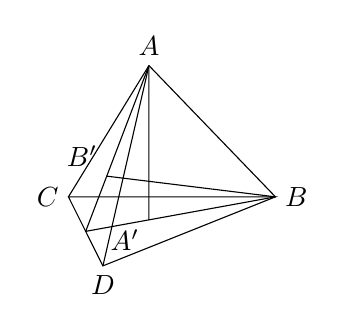
\begin{tikzpicture}[scale=0.8]
			          %projection ($(X)!(B')!(B)$)
			          %nommer chemin 'name path
			          %intersection \path [name intersections={of=d and gb,by=G}];
			          %TETRAEDRE 
				  \coordinate[label=above:$A$] (A) at (0,2.449,0);
				  \coordinate[label=right:$B$] (B) at (1.64317,0,-0.948683);
				  \coordinate[label=left:$C$] (C) at (-1.64317,0,-0.948683);				  
				  \coordinate[label=below:$D$] (D) at (0,0,1.89737);
				  \draw (B) -- (C) -- (D) -- cycle;
				  \draw (A) -- (B);
				  \draw (A) -- (C);
				  \draw (A) -- (D);
				  %A',B'
				  \coordinate[label=below left:$A'$] (A') at (0,0,0);
				  \coordinate[label=above left:$B'$](B') at ($0.333*(A)+0.333*(C)+0.333*(D)$);
				  %AA',BB'
				  \draw (A) -- (A') (B) -- (B');
				  
				  \coordinate[] (E) at ($0.5*(C)+0.5*(D)$); 
				  \draw (A) -- (E) -- (B);
				  \end{tikzpicture}
				  \end{figure}
			
				  \begin{tcolorbox}[basic] 
				      
				    \smallskip
				    \underline{Hypothèses} 
				    \begin{enumerate}
				    \item $AA'\bot BCD$,
				    \item $BB'\bot ACD$.
				    \end{enumerate}
							      
				    \underline{Thèse} 
				    \renewcommand{\theenumi}{\alph{enumi})}
				    \begin{enumerate}
				    \item $AA'\nmid BB' \leftrightarrow CD \orthog AB$,
				    \item côtés opposés $\orthog \rightarrow$ hauteurs concourantes.
				    \end{enumerate}
				    \end{tcolorbox}
		
		
		\column{.5\textwidth}\centering
		
		\underline{Résolution}\\ \flushleft
		$AA'\nmid BB' \rightarrow \exists \text{ plan } ABA'$ \\ \smallskip
		\heart Une droite est $\bot$ à un plan si elle est ortogonale à 2 droites sécantes de celui-ci.\\ \smallskip
		\begin{enumerate}
		 \item $CD \orthog AA'$,
		 \item $CD \orthog BB'$,
		\end{enumerate}
		$CD \bot ABA' \rightarrow AB\orthog CD$. \hfill $\qed (a\rightarrow)$ \\ \bigskip
		
		$CD \orthog AB$ et :
		\begin{enumerate}
		 \item $CD \orthog AA'$, $\rightarrow CD \bot AA'B$.
		 \item $CD \orthog BB'$, $\rightarrow CD \bot AB'B$.
		\end{enumerate} \smallskip
		\heart Il n'existe qu'un plan $\bot$ à une droite donnée passant par un point donné. \\ \medskip
		$B\in AA'B,AB'B \rightarrow AA'B=AB'B$
		
		
		%\centering\noindent\rule{2cm}{0.4pt}
	        %\hfill $\qed$

   
	   \end{columns}
    
    
    
    }
    
    \frame{ 
	  % résolution ex1
	  \begin{columns}[t]
		\column{.5\textwidth}\centering 
		

			\underline{Dessin}\\
			
				  \begin{figure}[h]
				  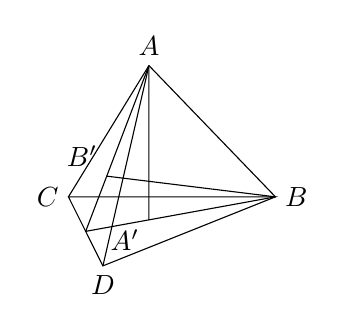
\begin{tikzpicture}[scale=0.8]
			          %projection ($(X)!(B')!(B)$)
			          %nommer chemin 'name path
			          %intersection \path [name intersections={of=d and gb,by=G}];
			          %TETRAEDRE 
				  \coordinate[label=above:$A$] (A) at (0,2.449,0);
				  \coordinate[label=right:$B$] (B) at (1.64317,0,-0.948683);
				  \coordinate[label=left:$C$] (C) at (-1.64317,0,-0.948683);				  
				  \coordinate[label=below:$D$] (D) at (0,0,1.89737);
				  \draw (B) -- (C) -- (D) -- cycle;
				  \draw (A) -- (B);
				  \draw (A) -- (C);
				  \draw (A) -- (D);
				  %A',B'
				  \coordinate[label=below left:$A'$] (A') at (0,0,0);
				  \coordinate[label=above left:$B'$](B') at ($0.333*(A)+0.333*(C)+0.333*(D)$);
				  %AA',BB'
				  \draw (A) -- (A') (B) -- (B');
				  
				  \coordinate[] (E) at ($0.5*(C)+0.5*(D)$); 
				  \draw (A) -- (E) -- (B);
				  \end{tikzpicture}
				  \end{figure}
			
				  \begin{tcolorbox}[basic] 
				      
				    \smallskip
				    \underline{Hypothèses} 
				    \begin{enumerate}
				    \item $AA'\bot BCD$,
				    \item $BB'\bot ACD$.
				    \end{enumerate}
							      
				    \underline{Thèse} 
				    \renewcommand{\theenumi}{\alph{enumi})}
				    \begin{enumerate}
				    \item $AA'\nmid BB' \leftrightarrow CD \orthog AB$,
				    \item côtés opposés $\orthog \rightarrow$ hauteurs concourantes.
				    \end{enumerate}
				    \end{tcolorbox}
		
		
		\column{.5\textwidth}\flushleft
		\heart 2 droites sont $\nmid$ si elles $\in$ au même plan et ne sont pas $\parallel$. \\ \medskip
		$AA'\nmid BB'.$ \hfill $\qed(a\leftarrow  )$ \\
		\centering\noindent\rule{2cm}{0.4pt} \\ \medskip \flushleft		
		De (a), côtés opposés $\orthog \rightarrow$ hauteurs deux à deux sécantes. \\
		\begin{numcases}{}X= AA' \cap BB', \label{eq:1}\\
					      Y= AA' \cap DD', \label{eq:2}\\
					      Z= BB' \cap DD'. \label{eq:3} 
			    \end{numcases} \smallskip
		
		 
		\begin{align*}
		Y \in& AA' \subset AA'B, \\
		Z \in& BB' \subset AA'B, \\
		\text{et }&  Y,Z \in DD', \\[1em]				
			    Y =& Z  =DD' \cap AA'B. \\[1.5em]					    	      
		\end{align*}
	        %\hfill $\qed$

   
	   \end{columns}
    
    
    
  }
  \frame{ 
	  % résolution ex1
	  \begin{columns}[t]
		\column{.5\textwidth}\centering 
		

			\underline{Dessin}\\
			
				  \begin{figure}[h]
				  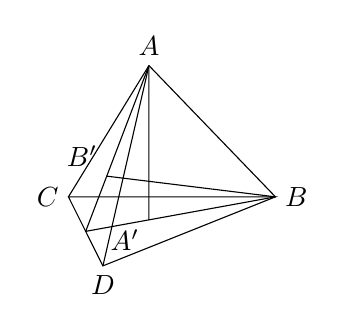
\begin{tikzpicture}[scale=0.8]
			          %projection ($(X)!(B')!(B)$)
			          %nommer chemin 'name path
			          %intersection \path [name intersections={of=d and gb,by=G}];
			          %TETRAEDRE 
				  \coordinate[label=above:$A$] (A) at (0,2.449,0);
				  \coordinate[label=right:$B$] (B) at (1.64317,0,-0.948683);
				  \coordinate[label=left:$C$] (C) at (-1.64317,0,-0.948683);				  
				  \coordinate[label=below:$D$] (D) at (0,0,1.89737);
				  \draw (B) -- (C) -- (D) -- cycle;
				  \draw (A) -- (B);
				  \draw (A) -- (C);
				  \draw (A) -- (D);
				  %A',B'
				  \coordinate[label=below left:$A'$] (A') at (0,0,0);
				  \coordinate[label=above left:$B'$](B') at ($0.333*(A)+0.333*(C)+0.333*(D)$);
				  %AA',BB'
				  \draw (A) -- (A') (B) -- (B');
				  
				  \coordinate[] (E) at ($0.5*(C)+0.5*(D)$); 
				  \draw (A) -- (E) -- (B);
				  \end{tikzpicture}
				  \end{figure}
			
				  \begin{tcolorbox}[basic] 
				      
				    \smallskip
				    \underline{Hypothèses} 
				    \begin{enumerate}
				    \item $AA'\bot BCD$,
				    \item $BB'\bot ACD$.
				    \end{enumerate}
							      
				    \underline{Thèse} 
				    \renewcommand{\theenumi}{\alph{enumi})}
				    \begin{enumerate}
				    \item $AA'\nmid BB' \leftrightarrow CD \orthog AB$,
				    \item côtés opposés $\orthog \rightarrow$ hauteurs concourantes.
				    \end{enumerate}
				    \end{tcolorbox}
		
		
		\column{.5\textwidth}\flushleft
		 
		\begin{align*}	
			    Y =& AA' \cap DD' = BB' \cap DD', (\ref{eq:2}=\ref{eq:3}) \\
			      =& AA' \cap BB', \text{(transitivité)}\\
			      =& X.\\
			    X =& Y = Z. 	      
		\end{align*} 
		
		\bigskip
		
		$AA',BB',DD'$ sont concourantes. \\ \medskip
		De la même façon : \\ \medskip
		$AA',BB',CC'$ sont concourantes. \\ \bigskip
		Ainsi $AA',BB',CC',DD'$ sont concourantes. \hfill $\qed$   
	   \end{columns}
    
    
    
  }
  
\end{document}
